\documentclass[../PianodiProgetto.tex]{subfiles}

\begin{document}
	
	\chapter{Introduzione}
	\section{Scopo del documento}
	Questo documento ha lo scopo di fornire le specifiche di pianificazione che il gruppo Graphite seguirà durante lo svolgimento del progetto. Nello specifico si prefigge di:
	
	\begin{itemize}
		\item Descrivere nel dettaglio la pianificazione dei tempi e delle \glossario{attività}{attivita};
		\item Fornire un preventivo delle risorse da utilizzare;
		\item Fornire il \glossario{consuntivo}{consuntivo} delle risorse;
		\item Analizzare i possibili fattori di rischio che potrebbero minare il corretto svolgimento del progetto.
	\end{itemize}
	
	\section{Scopo del prodotto}
	
	L'obiettivo di questo progetto è realizzare un'interfaccia grafica per Speect, una libreria per la creazione di sistemi di sintesi vocale, che agevoli l'ispezione del suo stato interno durante il funzionamento e la scrittura di test per le sue funzionalità.
	Nello specifico l'interfaccia dovrà avere le seguenti funzioni:
	\begin{itemize}
		\item Visualizzazione del \glossario{grafo HRG}{grafo HRG}, ovvero il grafo dei risultati delle componenti di analisi linguistica;
		\item Caricamento/Modifica/Salvataggio del grafo;
		\item Manipolazione della struttura dati interna e la configurazione di Speect;
		\item Caricamento ed esecuzione manuale di singole componenti di analisi;
		\item Manipolazione della struttura dati interna e della configurazione di Speect;
		\item Possibilità di visualizzare percorsi su un grafo;
		\item Possibilità di confrontare visivamente e/o automaticamente due stati della struttura interna di Speect;
		\item Permettere lo sviluppo di test in grado di caricare un particolare stato interno e verificare che gli effetti dell’esecuzione del plugin siano quelli attesi.
	\end{itemize}
	
	\noindent La progettazione e l'implementazione dovranno tener conto della manutenibilità e dell'estensibilità dell'applicazione, cercando di conciliare i vari casi d'uso (sviluppatore che vuole ispezionare lo stato interno della libreria, sviluppatore che vuole creare dei test, sviluppatore che vuole creare configurazioni particolari). 
	
	\section{Glossario}
	Al fine di evitare ogni ambiguità di linguaggio e massimizzare la comprensione dei documenti, i termini tecnici, di dominio, gli acronimi e le parole che necessitano di essere chiarite, sono riportate nel documento \textit{Glossario v1.0.0}. Ogni termine presente nel glossario è marcato da una "G" maiuscola in pedice.
	
	\section{Riferimenti}
	
	\subsection{Normativi}
	\begin{itemize}
		\item \textbf{Norme di Progetto:} \textit{Norme di Progetto v1.0.0};
		\item \textbf{\textit{Capitolato\ped{G}} d'appalto C3:}\\ \url{http://www.math.unipd.it/~tullio/IS-1/2017/Progetto/C3.pdf};
		\item \textbf{Regole del progetto:}\\ \url{http://www.math.unipd.it/~tullio/IS-1/2017/Dispense/P01.pdf};
		\item \textbf{Vincoli Organigramma e Offerta tecnico-economica:}\\ \url{http://www.math.unipd.it/~tullio/IS-1/2017/Progetto/RO.html}.
	\end{itemize}
	
	\subsection{Informativi}
	\begin{itemize}
		\item \textbf{Slide del corso:} \url{http://www.math.unipd.it/~tullio/IS-1/2017/};
		\item \textbf{Studio di Fattibilità:} \textit{Studio di Fattibilità v1.0.0};
		\item \textbf{Analisi dei Requisiti:} \textit{Analisi dei Requisiti v1.0.0}.
	\end{itemize}
	
	\section{Scadenze}
	Le scadenze che il gruppo Graphite ha deciso di rispettare sono le seguenti:
	\begin{itemize}
		\item \textbf{Revisione dei Requisiti(RR):} 26-01-2018;
		\item \textbf{Revisione di Progettazione(RP):} 19-03-2018;
		\item \textbf{Revisione di Qualifica(RQ):} 23-04-2018;
		\item \textbf{Revisione di Accettazione(RA):} 14-05-2018.
	\end{itemize}
	
	\chapter{Analisi dei rischi}
	
	\section{Visione generale dell'analisi dei rischi}
	
	Per una buona riuscita del \glossario{prodotto}{prodotto} è necessario effettuare un'approfondita analisi dei rischi che si possono incontrare durante lo svolgimento dell'intero progetto. I rischi vengono dunque brevemente descritti, analizzati per probabilità di frequenza e fattore di rischio e viene infine proposto un metodo di controllo e delle contromisure per ognuno di essi, i rischi effettivamente riscontrati vengono riportati in appendice §A "Rilevazione dei rischi" di questo documento.
	
	\section{Procedura di analisi dei rischi}
	
	La procedura utilizzata per l'analisi dei rischi è la seguente:
	
	\begin{enumerate}
		\item \textbf{Identificazione}: vengono individuati i potenziali rischi che si ritiene possano presentarsi durante
		l’avanzamento di un processo e se ne identifica la tipologia. I rischi possono essere inerenti a: 
		\begin{itemize}
			\item \textbf{Progetto}: relativi a pianificazione, strumenti, costi e risorse;
			\item \textbf{Prodotto}: relativi a conformità ai requisiti e alle aspettative del committente in termini qualitativi.
		\end{itemize}
		\item \textbf{Analisi}: valutazione della probabilità dell’occorrenza del rischio e delle possibili ricadute
		sul progetto di quest'ultima;
		\item \textbf{Pianificazione del controllo}: definizione di metodi di controllo dei rischi;
		\item \textbf{Mitigazione}: definizione di accorgimenti atti a mitigare gli effetti deleteri di un rischio nel caso in cui dovesse verificarsi. Ciò è richiesto solo per rischi
		difficilmente controllabili e gestibili.
	\end{enumerate}

	\section{Catalogazione dei rischi}
	
	Ogni rischio verrà catalogato secondo il seguente codice identificativo:
	
	\begin{center}
		R[Tipologia].[Identificativo]
	\end{center}

	Dove:
	\begin{itemize}
		\item \textbf{Tipologia}: indica il tipo di rischio in esame, e può assumere uno dei seguenti valori:
		\begin{itemize}
			\item \textbf{T}: rischi inerenti le tecnologie;
			\item \textbf{S}: rischi inerenti gli strumenti;
			\item \textbf{G}: rischi inerenti il gruppo di progetto;
			\item \textbf{R}: rischi inerenti i requisiti;
			\item \textbf{O}: rischi inerenti l'organizzazione.
		\end{itemize}
		\item \textbf{Identificativo}: indica un codice incrementale per il rischio.
	\end{itemize}

	Ogni rischio è inoltre corredato da:
	
	\begin{itemize}
		\item \textbf{Nome}: nome descrittivo del rischio;
		\item \textbf{Descrizione}: breve descrizione;
		\item \textbf{Probabilità di occorrenza}: indica la probabilità che il rischio si verifichi effettivamente;
		\item \textbf{Livello di gravità}: indica l'impatto che il verificarsi del rischi avrebbe sul progetto;
		\item \textbf{Strategia di rilevazione}: indica una possibile strategia con cui tracciare il rischio;
		\item \textbf{Contromisure}: indica eventuali contromisure per mitigare gli effetti deleteri del verificarsi del rischio.
	\end{itemize}
	
	\section{Descrizione dei rischi} 
	
	\subsection{Rischi legati alle tecnologie}
	
	\subsubsection{Inesperienza delle tecnologie da utilizzare}
	\begin{itemize}
		\item \textbf{Codice:} RT0;
		\item \textbf{Nome:} Inesperienza delle tecnologie da utilizzare;
		\item \textbf{Descrizione:} le tecnologie adottate per sviluppare il prodotto sono solamente in parte note ai componenti del gruppo, ciò non toglie che vi possano essere delle mancanze;
		\item \textbf{Probabilità di occorrenza:} bassa;
		\item \textbf{Livello di gravità:} medio-alto ;
		\item \textbf{Strategie di rilevazione:} il \textit{Responsabile} ha il compito di verificare il grado di conoscenza di ciascun componente, relativo alle tecnologie adottate;
		\item \textbf{Contromisure:} ciascun componente si impegnerà a documentarsi in maniera autonoma sulle tecnologie adottate. 
	\end{itemize}
	
	\subsection{Rischi legati agli strumenti}
	
	\subsubsection{Guasti hardware e problematiche software}
	\begin{itemize}
		\item \textbf{Codice:} RS0;
		\item \textbf{Nome:} Guasti hardware e problematiche software;
		\item \textbf{Descrizione:} la strumentazione usata dal gruppo potrebbe avere dei malfunzionamenti o guastarsi durante lo sviluppo del progetto, rendendo difficoltoso l'avanzamento del progetto o fermarlo;
		\item \textbf{Probabilità di occorrenza:} bassa;
		\item \textbf{Livello di gravità:} basso;
		\item \textbf{Strategie di rilevazione:} ogni membro deve aver cura della propria strumentazione;
		\item \textbf{Contromisure:} ogni componente del gruppo deve salvare il proprio lavoro sul \glossario{repository}{Repository} \glossario{GitHub}{GitHub} dedicato al progetto, se tale operazione non è possibile allora deve salvarlo su una periferica di archiviazione di massa esterna.
	\end{itemize}
	
	\subsubsection{Inesperienza degli strumenti da utilizzare}
	\begin{itemize}
		\item \textbf{Codice:} RS1;
		\item \textbf{Nome:} Inesperienza degli strumenti da utilizzare;
		\item \textbf{Descrizione:} l'approccio al metodo di lavoro risulta nuovo. Sono richieste capacità di pianificazione e di analisi che il gruppo non possiede a causa dell'inesperienza. Alcune conoscenze richieste richiedono tempo per essere apprese;
		\item \textbf{Probabilità di occorrenza:} alta;
		\item \textbf{Livello di gravità:} alto;
		\item \textbf{Strategie di rilevazione:} quando un componente del gruppo stabilisce che è necessario utilizzare un nuovo strumento lavorativo deve segnalarlo al  \textit{Responsabile}. Una volta approvato l'utilizzo di tale strumento, il gruppo si dovrà documentare su come impiegarlo;
		\item \textbf{Contromisure:} ogni membro del gruppo dovrà studiare tutto il materiale necessario per essere in grado di far fronte  a ciò che il progetto richiede.
	\end{itemize}
	
	\subsection{Rischi legati al gruppo di progetto}
	\subsubsection{Problemi personali dei membri del gruppo}
	\begin{itemize}
		\item \textbf{Codice:} RG0;
		\item \textbf{Nome:} Problemi personali dei membri del gruppo;
		\item \textbf{Descrizione:} ogni membro del gruppo ha degli impegni personali o potrebbe avere dei problemi di salute. Questo implica la possibilità che qualche componente non sia disponibile in certi momenti creando eventualmente dei rallentamenti al progetto;
		\item \textbf{Probabilità di occorrenza:} media;
		\item \textbf{Livello di gravità:} medio;
		\item \textbf{Strategie di rilevazione:} grazie alla compilazione di calendari di gruppo e ad una tempestiva comunicazione fra componenti, il \textit{Responsabile} sarà in grado di avere un quadro generale delle problematiche.
		\item \textbf{Contromisure:} Nel caso un componente del gruppo non sia disponibile per un breve periodo di tempo, egli dovrà comunicarlo tempestivamente al \textit{Responsabile}, il quale organizzerà e ripartirà il carico di lavoro ai rimanenti componenti del gruppo. 
	\end{itemize}
	
	\subsubsection{Problemi tra membri del gruppo}
	\begin{itemize}
		\item \textbf{Codice:} RG1;
		\item \textbf{Nome:} Problemi tra membri del gruppo;
		\item \textbf{Descrizione:} la maggior parte dei membri del gruppo non si conosceva prima di questo progetto. Questo può portare a delle incomprensioni causate anche da diversi punti di vista;
		\item \textbf{Probabilità di occorrenza:} bassa;
		\item \textbf{Livello di gravità:} alto;
		\item \textbf{Strategie di rilevazione:} il \textit{Responsabile} deve monitorare lo stato di collaborazione fra i vari componenti del gruppo durante le varie fasi e capire dove stia nascendo un dissidio fra uno o più membri;
		\item \textbf{Contromisure:} Nel caso si verifichino forti dissidi, il \textit{Responsabile} dovrà prendere in mano la situazione e cercare di trovare una soluzione di comune accordo con i membri in contrasto. 
	\end{itemize}
	
	\subsection{Rischi legati ai requisiti}
	\subsubsection{Comprensione dei requisiti}
	\begin{itemize}
		\item \textbf{Codice:} RR0;
		\item \textbf{Nome:} Comprensione dei requisiti;
		\item \textbf{Descrizione:} data l'inesperienza dei componenti del gruppo nell'analisi dei requisiti, è possibile un'errata comprensione dei requisiti comportando un'offerta non conforme alle richieste;
		\item \textbf{Probabilità di occorrenza:} medio-bassa;
		\item \textbf{Livello di gravità:} alto;
		\item \textbf{Strategia di rilevazione:} per ridurre al minimo gli errori dell'analisi, è utile organizzare incontri con il proponente al fine di sciogliere ogni dubbio e capire a fondo le sue esigenze;
		\item \textbf{Contromisure:} organizzare incontri col proponente permetterà al gruppo di capire con maggior chiarezza i requisiti necessari. Inoltre è importante correggere tempestivamente ogni errore e imprecisione individuati alle revisioni. 
	\end{itemize}
	
	\subsection{Rischi legati all'organizzazione}
	\subsubsection{Sottostima dei tempi necessari}
	\begin{itemize}
		\item \textbf{Codice:} RO0;
		\item \textbf{Nome:} Sottostima dei tempi necessari;
		\item \textbf{Descrizione:} data l'inesperienza dei componenti del gruppo nella pianificazione di progetto e l'attuazione della stessa su una arco di tempo medio-lungo, può verificarsi la sottostima dei tempi necessari alla realizzazione del progetto;
		\item \textbf{Probabilità di occorrenza:} media;
		\item \textbf{Livello di gravità:} alto;
		\item \textbf{Strategia di rilevazione:} ogni componente del gruppo controllerà periodicamente lo stato della propria attività rispetto alla tabella di marcia imposta nella pianificazione;
		\item \textbf{Contromisure:} per ogni attività, è previsto un tempo di \glossario{slack}{Slack}, in modo che un ritardo non incida negativamente nell'avanzamento del progetto.
	\end{itemize}

	\chapter{Ciclo di vita}

	Il modello di ciclo di vita adottato dal gruppo è il \glossario{modello incrementale}{modello incrementale}. Le motivazioni che hanno portato alla scelta di questo modello sono:
	\begin{itemize}
		\item Possibilità di suddividere il lavoro in più sottoattività sviluppate in modo parallelo. Questo permette maggior controllo sull’avanzamento del progetto;
		\item Lo sviluppo avviene per incrementi, dove ogni incremento rilascia parte delle funzionalità richieste;
		\item I requisiti vengono suddivisi in livelli di priorità. Quelli a priorità maggiore verranno soddisfatti con i primi incrementi, questo permette più attività di verifica e quindi maggiore stabilità ad ogni iterazione;
		\item I primi incrementi possono essere usati come prototipo per aiutare a definire i requisiti degli incrementi successivi;
		\item Minimizzare i rischi di ritardo rispetto ai tempi stabiliti in quanto i cicli hanno durata breve e sono precedentemente pianificati.
	\end{itemize}
	Alla fine della prima fase si avrà un prototipo funzionante con le implementazioni dei requisiti obbligatori. Tramite incrementi successivi verranno integrate le funzionalità opzionali.
	
	\chapter{Pianificazione}
	
	La pianificazione del lavoro stata costruita sulla base delle scadenze elencate alla sezione 2.5 del seguente documento. In base ad esse, si è suddiviso lo sviluppo in cinque periodi. I periodi scelti sono i seguenti:
	\begin{itemize}
		\item Analisi;
		\item Consolidamento dei requisiti;
		\item Progettazione architetturale;
		\item Progettazione di dettaglio e Codifica;
		\item Validazione e collaudo.
	\end{itemize}

	\section{Analisi}
	Inizia il 07-11-2017 con la formazione del gruppo e termina il 16-01-2018 con la scadenza per la consegna dei documenti relativi alla Revisione dei Requisiti.
	Durante questa attività vengono svolte le seguenti sotto-attività:
	\begin{itemize}
		\item \textbf{Norme di Progetto:} vengono individuate dal gruppo tutte le norme e gli strumenti per il corretto svolgimento del progetto, riportando il tutto nel documento \textit{Norme di Progetto};
		\item \textbf{Studio di Fattibilità:} in questa attività vengono studiati i vari capitolati, analizzando i vari pro e contro, scegliendo quale sviluppare, lo studio fatto viene tradotto in forma scritta nel documento \textit{Studio di Fattibilità};
		\item \textbf{Analisi dei Requisiti:} viene effettuata un'analisi approfondita dei requisiti del capitolato che il gruppo ha deciso di sviluppare, il tutto riportato nel documento \textit{Analisi dei Requisiti};
		\item \textbf{Piano di Progetto:} durante questa attività vengono individuate e pianificate le varie attività da svolgere per la realizzazione del progetto suddividendo le risorse disponibili, tutto ciò viene formalizzato nel documento \textit{Piano di Progetto}; 
		\item \textbf{Piano di Qualifica:} vengono definite le metriche per il prodotto, le quali vengono riportate nel \textit{Piano di Qualifica};
		\item \textbf{Glossario:} viene redatto il documento \textit{Glossario}	contenente tutti i termini tecnici, di dominio, gli acronimi e le parole che necessitano di essere chiarite per migliorare la comprensione dei documenti;
		\item \textbf{Lettera di Presentazione:} viene redatta la \textit{Lettera di Presentazione} per presentare la candidatura del gruppo.	
	\end{itemize}
	
	\subsection{Analisi - Diagramma di Gantt}
	\begin{figure}[H]
		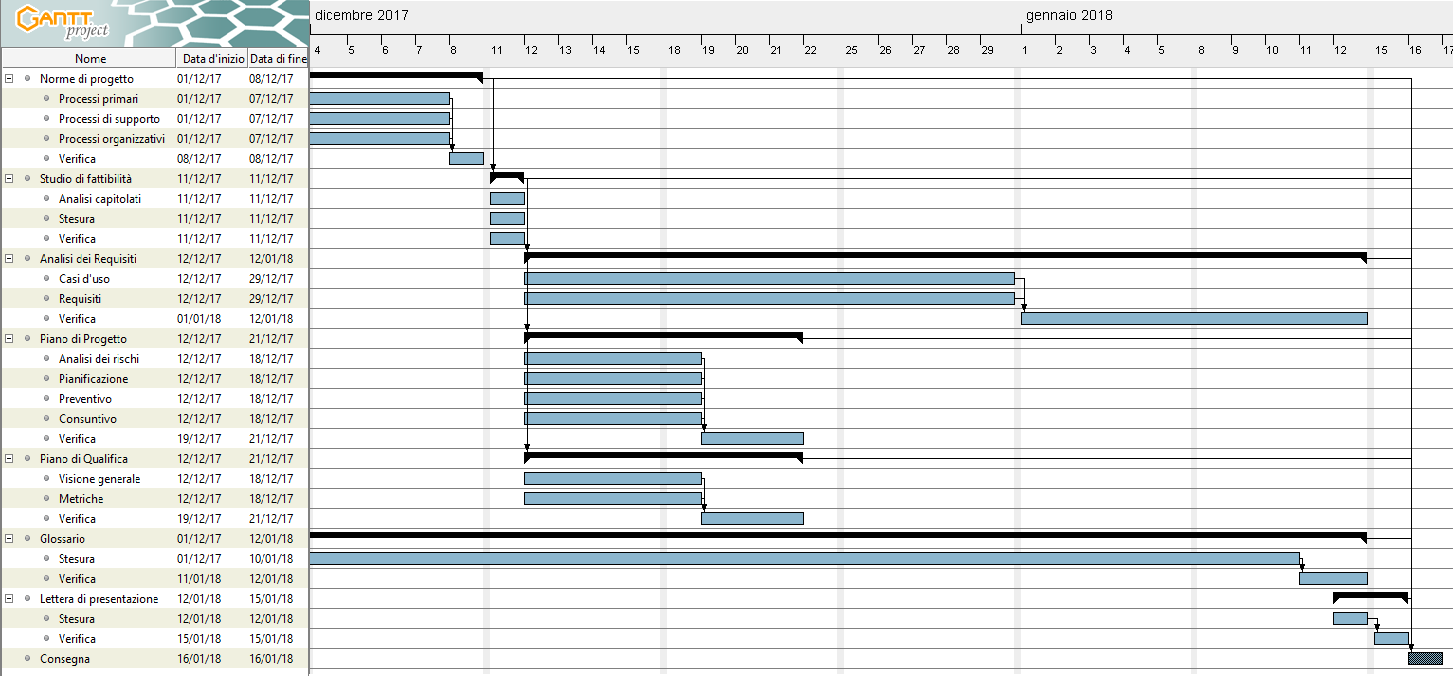
\includegraphics[width=1\linewidth]{AnalisiGantt.png}	
		\caption{Diagramma di Gantt di Analisi}\label{fig:1}	
	\end{figure}
	\newpage
	\section{Consolidamento dei requisiti} Inizia dopo la consegna dei documenti per la Revisione dei Requisiti e termina con la presentazione della Revisione dei Requisiti il 26-01-2018. Questa attività consiste nel migliorare e consolidare quanto fatto nell'Analisi dei Requisiti.
	\subsection{Consolidamento dei requisiti - Diagramma di Gantt}
	\begin{figure}[H]
		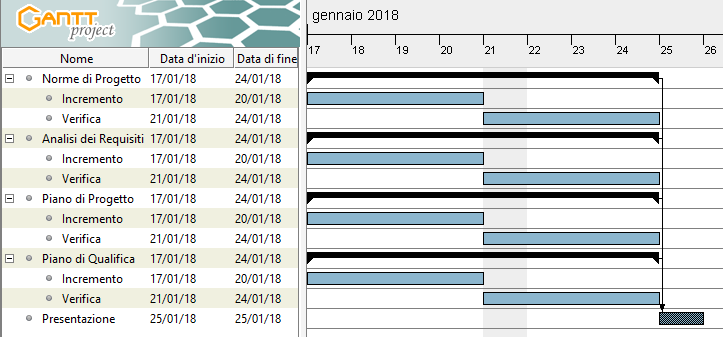
\includegraphics[width=\linewidth]{ConsolidamentoGantt.png}	
		\caption{Diagramma di Gantt di Consolidamento dei requisiti}\label{fig:2}
	\end{figure}
	\newpage
	\section{Progettazione architetturale}
	Inizia dopo la presentazione della Revisione dei Requisiti e termina il 19-03-2018 con la Revisione di Progettazione.
	Durante questa attività vengono svolte le seguenti sotto-attività:
	\begin{itemize}	
		\item \textbf{Incrementazione e Verifica}: vengono incrementati e verificati, se necessario, i documenti già redatti, correggendo i difetti emersi nell'esito della Revisione dei Requisiti;
		\item \textbf{Specifica Tecnica:} viene individuata l'architettura di alto livello per la realizzazione del prodotto, il documento \textit{Specifica Tecnica} contiene la descrizione dettagliata di essa;
		\item \textbf{Glossario:} vengono inseriti nuovi termini nel \textit{Glossario} e, se necessario, viene migliorato.
	\end{itemize}
	
	\subsection{Progettazione architetturale - Diagramma di Gantt}
	\begin{figure}[H]
		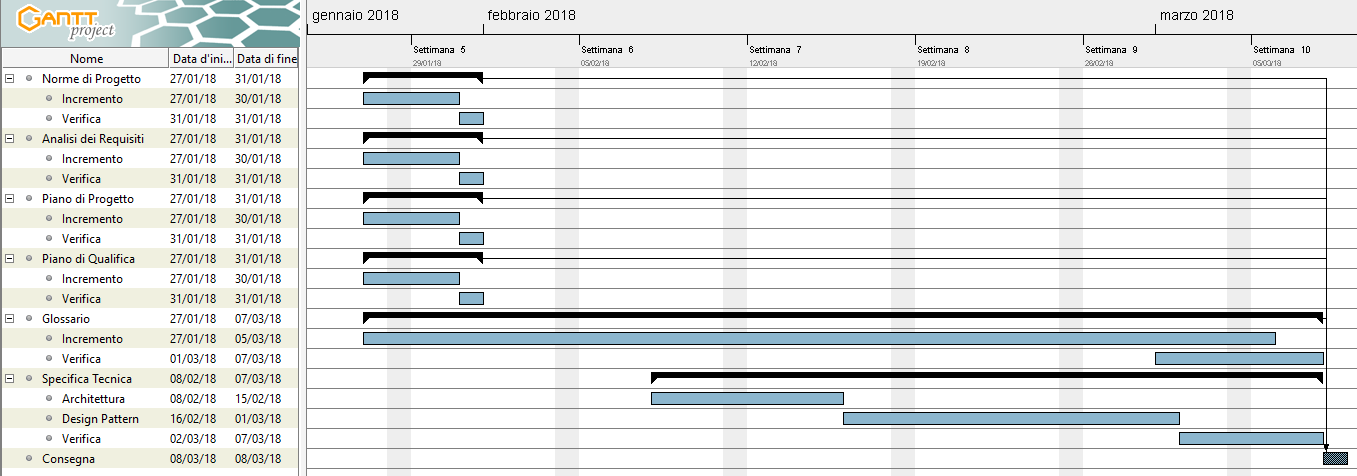
\includegraphics[width=\linewidth]{ProgArchitetturale.png}	
		\caption{Diagramma di Gantt di Progettazione architetturale}\label{fig:3}
	\end{figure}
	\newpage
	\section{Progettazione di dettaglio e Codifica}
	Inizia dopo la Revisione di Progettazione e termina con la Revisione di Qualifica del 23-04-2018. Durante questa attività vengono svolte le seguenti sotto-attività:
	\begin{itemize}
		\item \textbf{Incrementazione e Verifica}: vengono incrementati e verificati, se necessario, i documenti già redatti, correggendo i difetti emersi nell'esito della Revisione di Progettazione;	
		\item \textbf{Definizione di Prodotto:} viene definita nel dettaglio la struttura e il funzionamento del prodotto per la sua codifica, descrivendola nel documento \textit{Definizione di Prodotto};
		\item \textbf{Codifica:} consiste nella stesura del codice per la creazione del prodotto;
		\item \textbf{Manuale Utente:} viene redatto il documento \textit{Manuale Utente}, contente indicazioni sul corretto utilizzo del prodotto; 
		\item \textbf{Glossario:} vengono inseriti nuovi termini nel \textit{Glossario} e, se necessario, viene migliorato.
	\end{itemize}
	\subsection{Progettazione di dettaglio e Codifica - Diagramma di Gantt}
	\begin{figure}[H]
		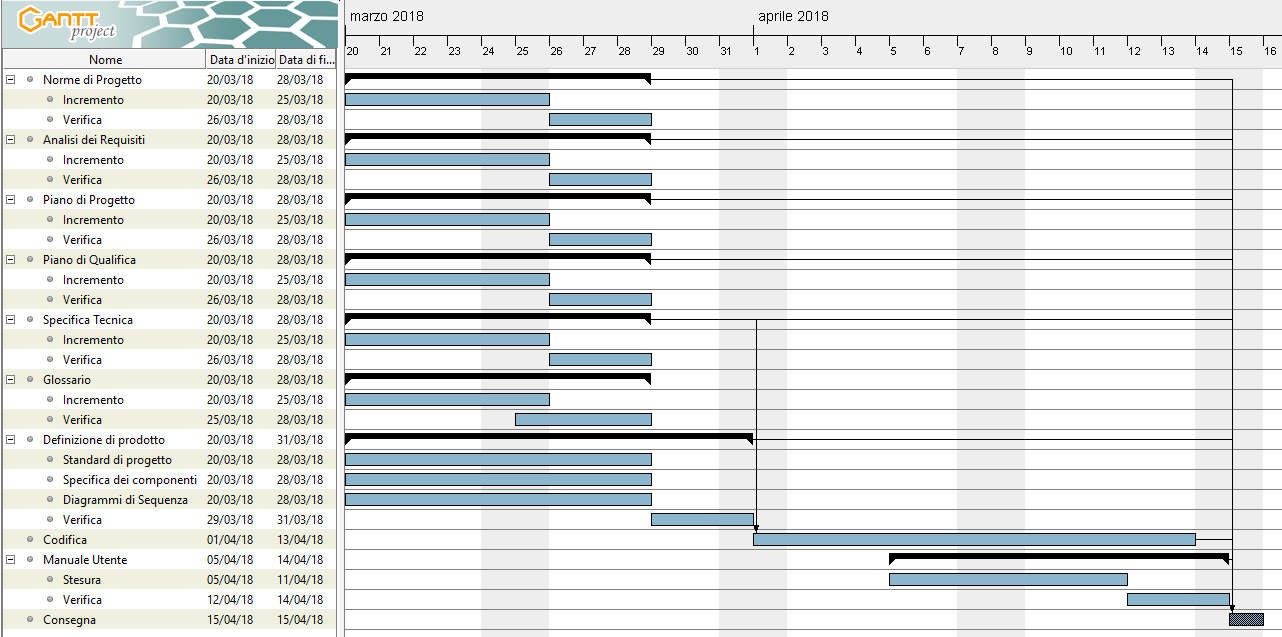
\includegraphics[width=\linewidth]{ProgCodifica.png}	
		\caption{Diagramma di Gantt di Progettazione di dettaglio e Codifica}\label{fig:4}	
	\end{figure}
	
	\section{Validazione e collaudo}
	Inizia dopo la Revisione di Qualifica e termina con la Revisione di Accettazione del 14-05-2018. Durante questa attività vengono svolte le seguenti sotto-attività:
	\begin{itemize}
		\item \textbf{Incrementazione e Verifica}: vengono incrementati e verificati, se necessario, i documenti già redatti, correggendo i difetti emersi nell'esito della Revisione di Qualifica;		
		\item \textbf{Validazione e Collaudo:} viene verificata la conformità del prodotto rispetto ai requisiti, testandolo per assicurarsi il corretto funzionamento ed il raggiungimento di determinati vincoli qualificativi.
		\item \textbf{Glossario:} vengono inseriti nuovi termini nel \textit{Glossario} e, se necessario, viene migliorato.
	\end{itemize}
	\subsection{Validazione e collaudo - Diagramma di Gantt}
	\begin{figure}[H]
		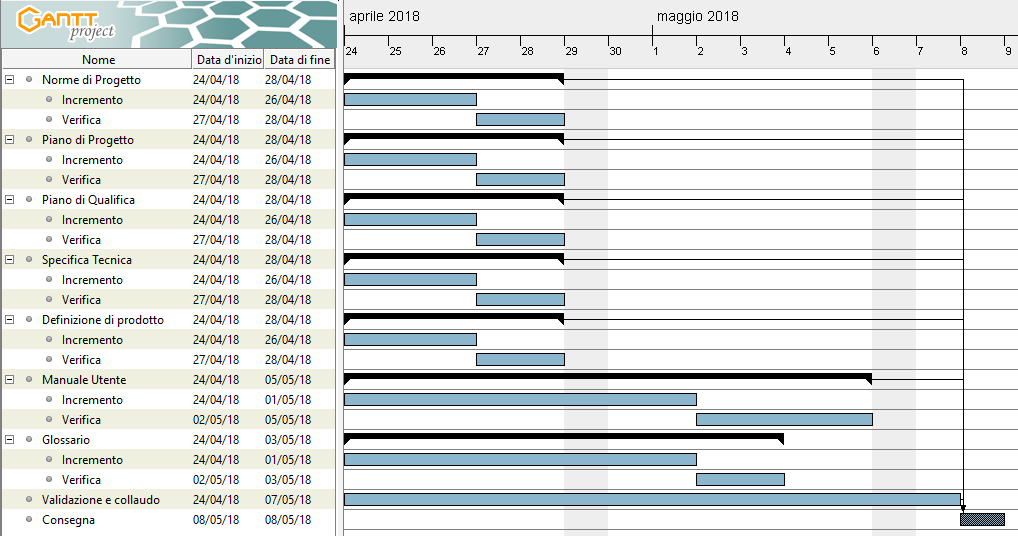
\includegraphics[width=\linewidth]{ValidazioneCollaudo.png}	
		\caption{Diagramma di Gantt di Validazione e collaudo}\label{fig:5}	
	\end{figure}

\end{document}